\begin{frame}
    \frametitle{Implementation}
    \framesubtitle{Integrators details}

    %\begin{columns}
    %    \begin{column}{0.5\textwidth}
            \begin{itemize}
                \item The code structure,
                \item Integration scheme,
                \item Parallelization scheme.
            \end{itemize}
    %    \end{column}

    %    \begin{column}{0.5\textwidth}
    %        \begin{Huge}
    %            \GR
    %        \end{Huge}
    %    \end{column}

    %\end{columns}

\end{frame}

%%%%%%%%%%%%%%%%%%%%%%%%%%%%%%%%%%%%%%%%%%%%%%%% CODE
%\section{The \GR\ code}
%\label{sec:code}
%\input{src/code}

\begin{frame}
    \frametitle{Implementation}
    \framesubtitle{The code}

    \begin{itemize}
        \item Main goal in the development, \blue{legibility}.
        \begin{itemize}
            \item Easy to read, modify and understand,
        \end{itemize}
        \item \blue{Balance} between optimization and maintainability.
    \end{itemize}


\end{frame}


\begin{frame}
    \frametitle{Implementation}
    \framesubtitle{The code}

    For the development of \GR, we have followed the next steps:

    \begin{itemize}
        \item Serial implementation,
        \item Profiling and performance assessment,
        \item Parallelization of the hot-spots,
        \item Optimization,
    \end{itemize}

    \begin{block}{\red{Note}}
        The same as CUDA C Best Practices~\cite{cudaBestPractices},
        called the APOD cycle, (Assess, Parallelize, Optimize and Deploy).
    \end{block}
\end{frame}


\begin{frame}
    \frametitle{Implementation}
    \framesubtitle{The code}

    \begin{itemize}
        \item OOP and SoA.
        \item Double-precision, importance of accuracy.
        \begin{itemize}
            \item on GPU, this reach the half of the theoretical maximum performance peak.
            \item NVIDIA Tesla C2050/M2050, single precision peak in GFLOPs is $1030.46$,
            and only $515.2$ with double precision.
        \end{itemize}
    \end{itemize}

    \begin{block}{\red{Note}}
        A posible future upgrade is to use mixed-precision~\cite{Aarseth85},
        or pseudo double-precision~\cite{keigo} to achieve a better performance
        in our code.
    \end{block}

\end{frame}

%%%%%%%%%%%%%%%%%%%%%%%%%%%%%%%%%%%%%% Integration scheme
%\section{Integration scheme}
%\label{sec:hermite}
%\input{src/hermite}

\begin{frame}
    \frametitle{Prediction-correction method}
    \framesubtitle{Introduction}
    \begin{columns}
        \begin{column}{0.6\textwidth}
            \begin{block}{In a {\nbody} system}
                The force acting on each particle varies smoothly.
            \end{block}

            \begin{itemize}
                \item Interpolation for the time interval extension (prediction).
                \item Reduce the amount of the force calculation.
                \item By finite differences it is possible to get the higher order
                derivatives of the force, which are used to add precision (correction).
            \end{itemize}
        \end{column}
        \begin{column}{0.4\textwidth}
            \begin{figure}
                \centering
                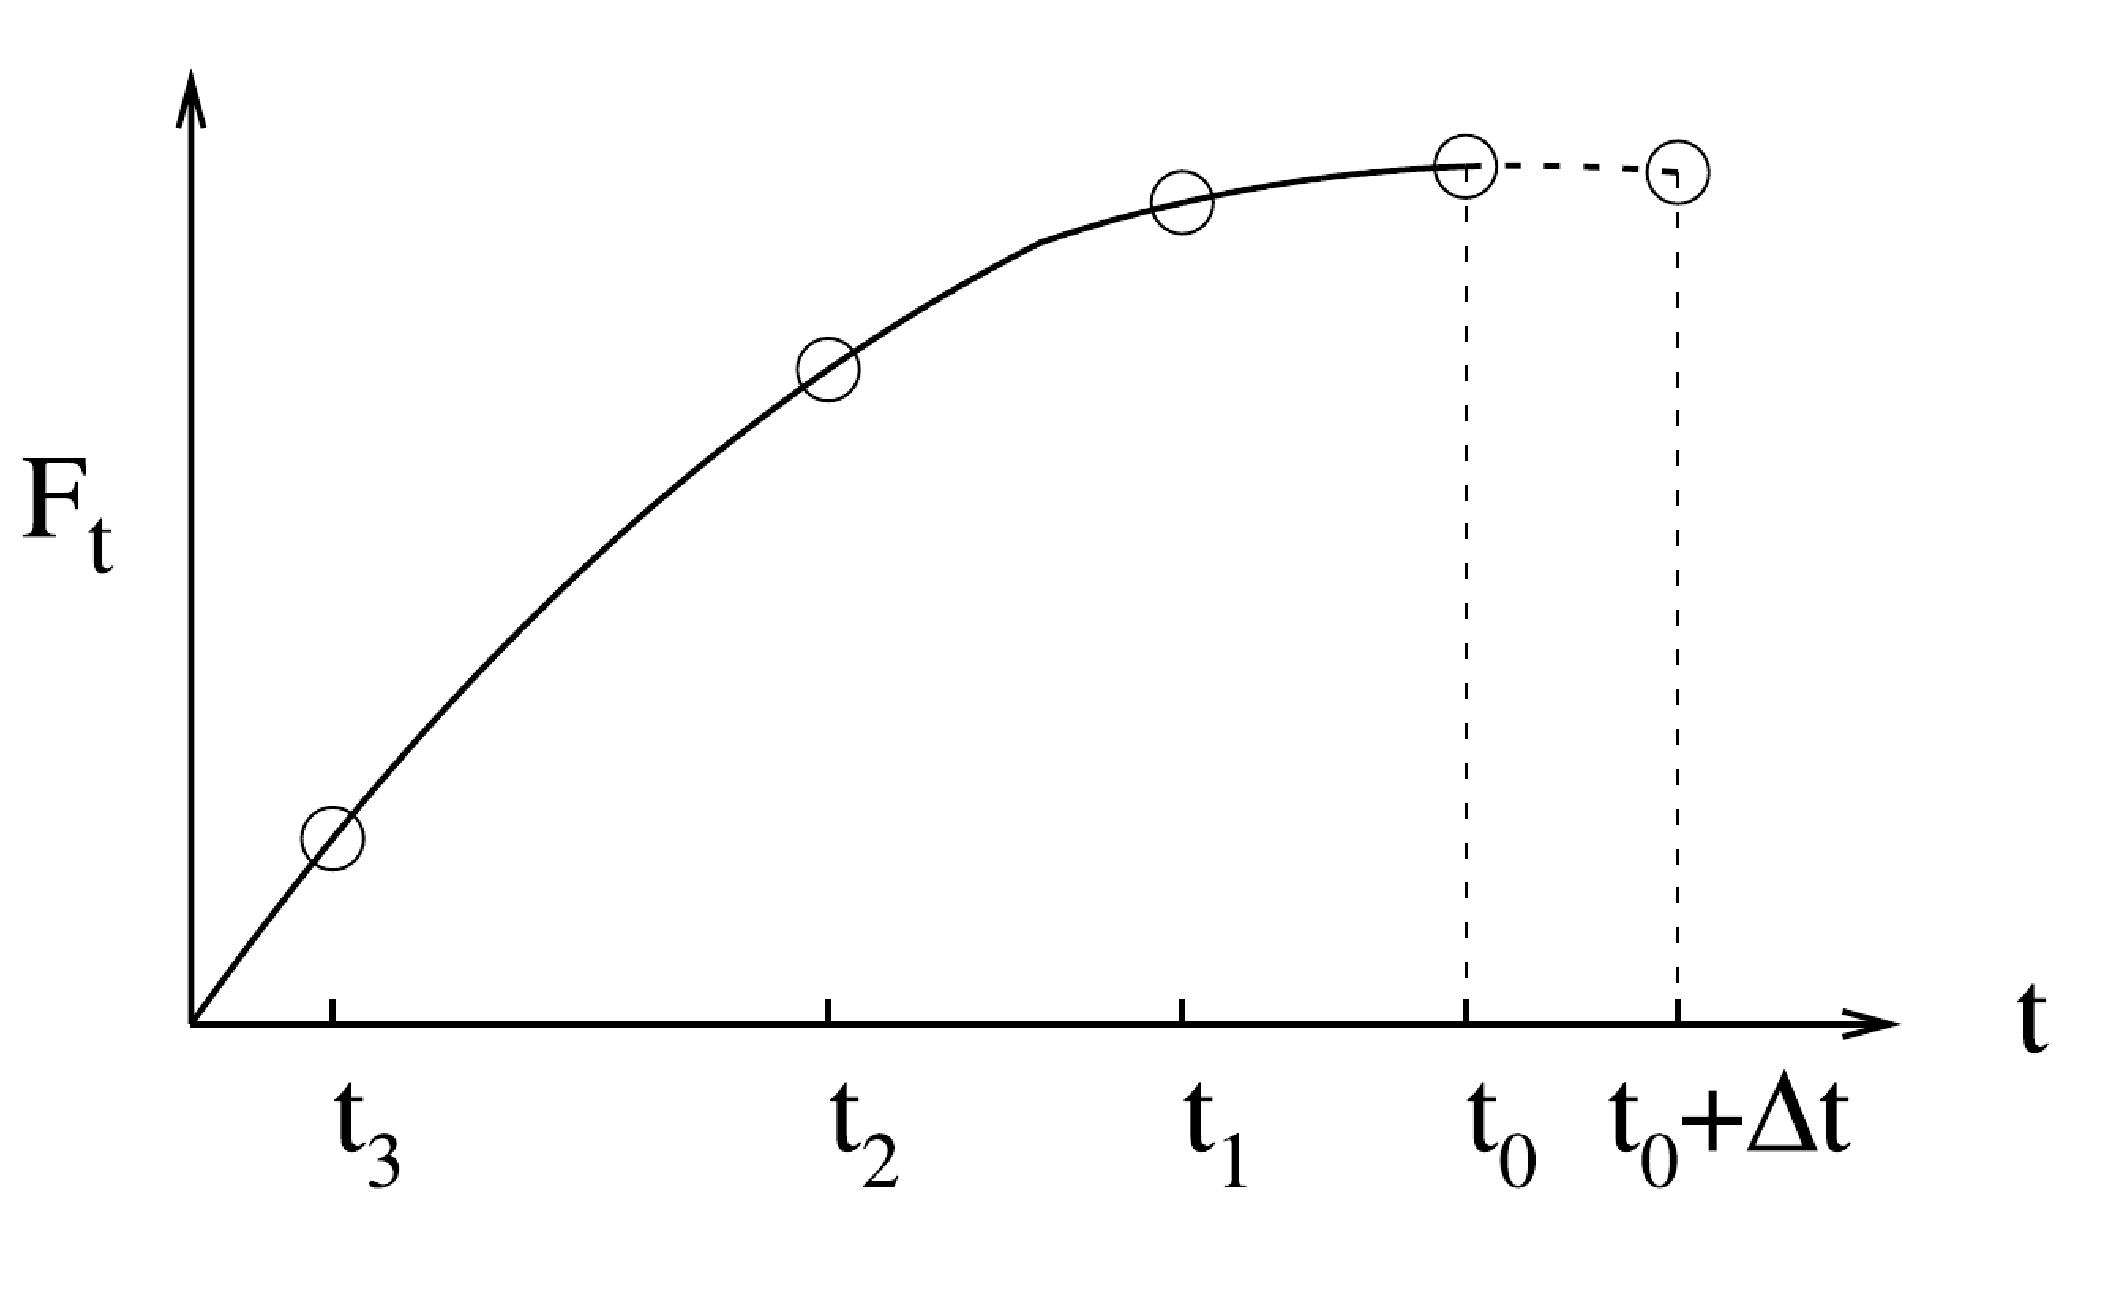
\includegraphics[width=0.8\textwidth]{img/polinomio}
                \caption{Polynomial fit of the gravitational force in function of time.}
                \label{fig:polinomio}
            \end{figure}

        \end{column}
    \end{columns}
\end{frame}

\begin{frame}[fragile]
    \frametitle{Prediction-correction method}
    \framesubtitle{Block time steps}
    \begin{columns}
        \begin{column}{0.6\textwidth}
            \begin{itemize}
                \item Reduce the amount of predictions,
                \item Enhance the parallelism,
                \item Based on an adaptive system.
                \begin{footnotesize}
                    \begin{dmath}
                        \Delta t_{i} = \sqrt{\eta  \frac{|\bs{a}_{i}|
                                                             |\bs{a}_{i}^{(2)}| +
                                                             |\bs{a}^{(1)}_{i}|^{2}}
                                                            {|\bs{a}^{(1)}_{i}|
                                                             |\bs{a}_{i}^{(3)}| +
                                                             |\bs{a}_{i}^{(2)}|^{2}}
                                                },\\
                    \end{dmath}
                \end{footnotesize}
            \end{itemize}

            \begin{small}
                \begin{block}{Block definition}
                    $2^{n} \Delta t_{s} \leq \Delta t_{i}\ $\textless$\ 2^{n+1} \Delta t_{s}$
                \end{block}
            \end{small}
        \end{column}
        \begin{column}{0.4\textwidth}
            \begin{figure}
                \centering
                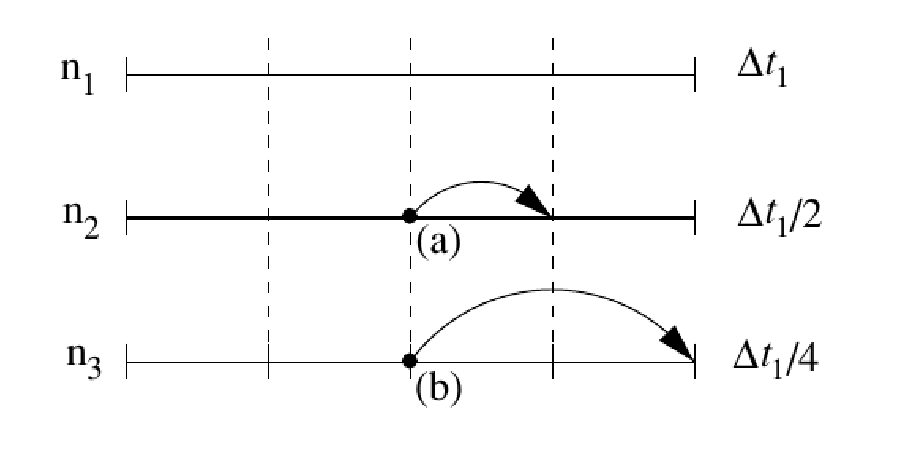
\includegraphics[width=0.9\textwidth]{img/blockdt}
                \caption{Time step hierarchical levels.}
                \label{fig:blockdt}
            \end{figure}
        \end{column}
    \end{columns}
\end{frame}

\begin{frame}
    \frametitle{Prediction-correction method}
    \framesubtitle{Hermite scheme}
    \begin{columns}
        \begin{column}{0.5\textwidth}
        \begin{block}{Prediction}
        \footnotesize
        \begin{dmath}
            \bs{r}_{i,pred} = \bs{r}_{i,0} +
                            \bs{v}_{i,0} \Delta t_{i}  +
                            \frac{1}{2!} \bs{a}_{i,0} \Delta t^{2}_{i} +
                            \frac{1}{3!} \bs{\dot{a}}_{i,0} \Delta t^{3}_{i}
        \end{dmath}
        \begin{dmath}
            \bs{v}_{i,pred} = \bs{v}_{i,0} +
                            \bs{a}_{i,0} \Delta t_{i}  +
                            \frac{1}{2!} \bs{\dot{a}}_{i,0} \Delta t^{2}_{i}
        \end{dmath}

        \end{block}
        \end{column}
        \begin{column}{0.5\textwidth}
            \begin{figure}
                \centering
                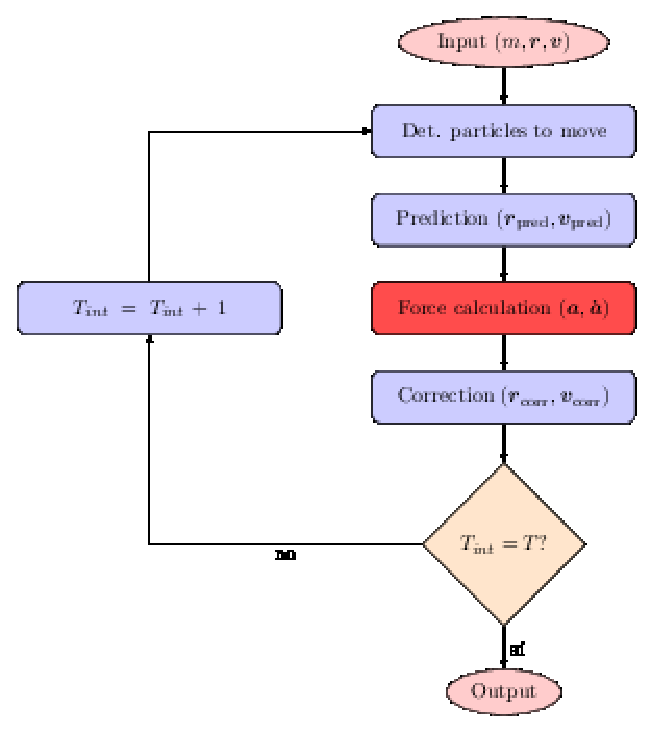
\includegraphics[height=0.7\textheight]{diagrams/algorithm}
                %\caption{}
                \label{fig:algoritmo}
            \end{figure}
        \end{column}
    \end{columns}
\end{frame}


\begin{frame}
    \frametitle{Prediction-correction method}
    \framesubtitle{Hermite scheme}
    \begin{columns}
        \begin{column}{0.5\textwidth}
            \begin{block}{Force calculation}
                \footnotesize
                \begin{dmath}
                    \bs{a}_{i,1} = \sum_{\substack{j=0\\j\neq i}}^{N} G m_{j}
                                    \frac{\bs{r}_{ij}}
                                           {(r_{ij}^2 + \epsilon^{2})^{\frac{3}{2}}}, \\
                \end{dmath}
                \begin{dmath}
                    \bs{\dot{a}}_{i,1} = \sum_{\substack{j=0\\j\neq i}}^{N} G m_{j}
                                    \left[
                                        \frac{\bs{v}_{ij}}
                                            {(r_{ij}^2 + \epsilon^{2})^{\frac{3}{2}}} -
                                        \frac{3(\bs{v}_{ij}\cdot \bs{r}_{ij}) \bs{r}_{i}}
                                            {(r_{ij}^2 + \epsilon^{2})^{\frac{5}{2}}}
                                    \right],
                \end{dmath}
            \end{block}
        \end{column}
        \begin{column}{0.5\textwidth}
            \begin{figure}
                \centering
                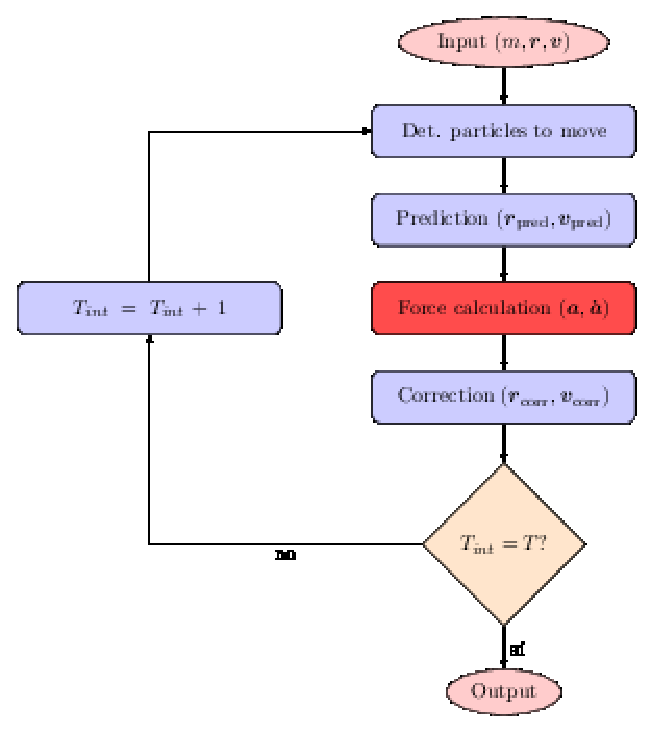
\includegraphics[height=0.7\textheight]{diagrams/algorithm}
                %\caption{}
                \label{fig:algoritmo}
            \end{figure}
        \end{column}
    \end{columns}
\end{frame}

\begin{frame}
    \frametitle{Prediction-correction method}
    \framesubtitle{Hermite scheme}
    \begin{columns}
        \begin{column}{0.5\textwidth}
        \begin{block}{Correction}
        \small
        \begin{dmath}
            \bs{r}_{i,1} = \bs{r}_{i,pred} +
                                \frac{1}{24}  \Delta t_{i}^{4} \bs{a}_{i,0}^{(2)} +
                                \frac{1}{120} \Delta t_{i}^{5} \bs{a}_{i,0}^{(3)} \\
        \end{dmath}
        \begin{dmath}
            \bs{v}_{i,1} = \bs{v}_{i,pred} +
                                \frac{1}{4}  \Delta t_{i}^{3} \bs{a}_{i,0}^{(2)} +
                                \frac{1}{24} \Delta t_{i}^{4} \bs{a}_{i,0}^{(3)}
        \end{dmath}

        \end{block}
        \end{column}
        \begin{column}{0.5\textwidth}
            \begin{figure}
                \centering
                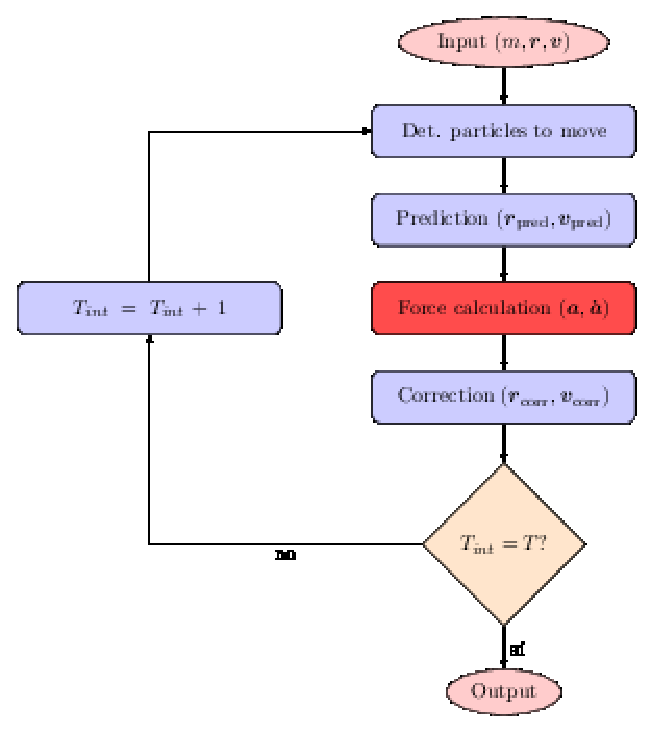
\includegraphics[height=0.7\textheight]{diagrams/algorithm}
                %\caption{}
                \label{fig:algoritmo}
            \end{figure}
        \end{column}
    \end{columns}
\end{frame}


%%%%%%%%%%%%%%%%%%%%%%%%%%%%%%%%%%%%%%%%%%%%%%%%%%%%%
%\section{The parallelization scheme}
%\label{sec:parallel}
%\input{src/parallel}

\begin{frame}
    \frametitle{Parallelization scheme}
    \framesubtitle{Force calculation}

    \begin{center}
    \begin{figure}[H]
        \centering
        \includegraphics[width=0.6\textwidth]{img/force_calculation.pdf}
        \caption{Force calculation code illustration.
                 The process itself belongs to a second level \texttt{for} loop.
                 Thanks to the integrator scheme, we have a reduction
                 of the step complexity from $O(N^{2})$ to $O(N_{act} N)$}
        \label{fig:force_code_diagram}
    \end{figure}
    \end{center}

\end{frame}

\begin{frame}
    \frametitle{Parallelization scheme}
    \framesubtitle{Calculation relations}

    \begin{center}
    \begin{figure}[H]
        \centering
        \includegraphics[width=0.7\textwidth]{img/forces_nact_n.pdf}
        \caption{Relation between the particles which will be updated in a certain
                 integration time ($N_{\rm act}$) and the whole set of particles ($N$).
                 The relation between the active particles and the others is
                 $N_{\rm act} << N$}
        \label{fig:nact_n}
    \end{figure}
    \end{center}

\end{frame}

\begin{frame}
    \frametitle{Parallelization scheme}
    \framesubtitle{Threads task}

    \begin{center}
    \begin{figure}[H]
        \centering
        \includegraphics[width=0.6\textwidth]{img/force_nact.pdf}
        \caption{For each $i-$particle in $N_{\rm act}$ a \texttt{for} will be through
                 the whole set of particles and perform the calculation of the
                 gravitational interaction between $i$ and $N$ particles.
                 The scheme could be know as $i-$parallelization, since it assumes
                 that each thread will be one $N_{\rm act}$
                 particle.}
        \label{fig:force_nact}
    \end{figure}
    \end{center}

\end{frame}

\begin{frame}
    \frametitle{Parallelization scheme}
    \framesubtitle{Tiles scheme}

    \begin{center}
    \begin{figure}[H]
        \centering
        \includegraphics[width=0.45\textwidth]{img/tiles.pdf}
        \caption{Grid configuration using the \emph{tiles} approach (This figure
        is based on~\cite{gpuGems3})}
        \label{fig:tile}
    \end{figure}
    \end{center}

\end{frame}

\begin{frame}
    \frametitle{Parallelization scheme}
    \framesubtitle{$j-$parallelization scheme}

    Our configuration is based in the idea presented in~\cite{NitadoriAarseth2012},

    \begin{center}
    \begin{figure}[H]
        \centering
        \includegraphics[width=0.55\textwidth]{img/force_split_reduction.pdf}
        \caption{Parallelization scheme to split the $j-$loop instead of the $i-$loop.
                 In this case, we have two sections, the first is to calculate
                 the force interactions of the $i-$particle with the whole
                 system but by different threads. Then a reduction (sum) is necessary
                 to get the new value for the $i-$particle force.}
        \label{fig:force_split_reduction}
    \end{figure}
    \end{center}

\end{frame}

